%!TEX root = main.tex
We consider a mmWave IAB network that consists of a mmWave BS,\textit{ IAB-donor}, connected to the core network through a wired connection, and a set of small mmWave BSs,\textit{ IAB-nodes}, wirelessly backhauled to the IAB-donor using mmWave frequencies.
Mobile UEs that move in the service area according to the well-known Random Waypoint model \cite{bai2004survey} get access to the network via either direct mmWave links connected with the IAB-donor or multiple hops through IAB-nodes. An example of IAB network scenario is depicted in Fig. \ref{fig:scenario}.
Backhaul links are established either between the IAB-donor and an IAB-node or between two IAB-nodes, while access links connect IAB-donor/IAB-nodes to UEs. Both backhaul and access transmissions share the same mmWave frequency band (i.e., in-band backhaul).

\begin{figure}
	\centering
	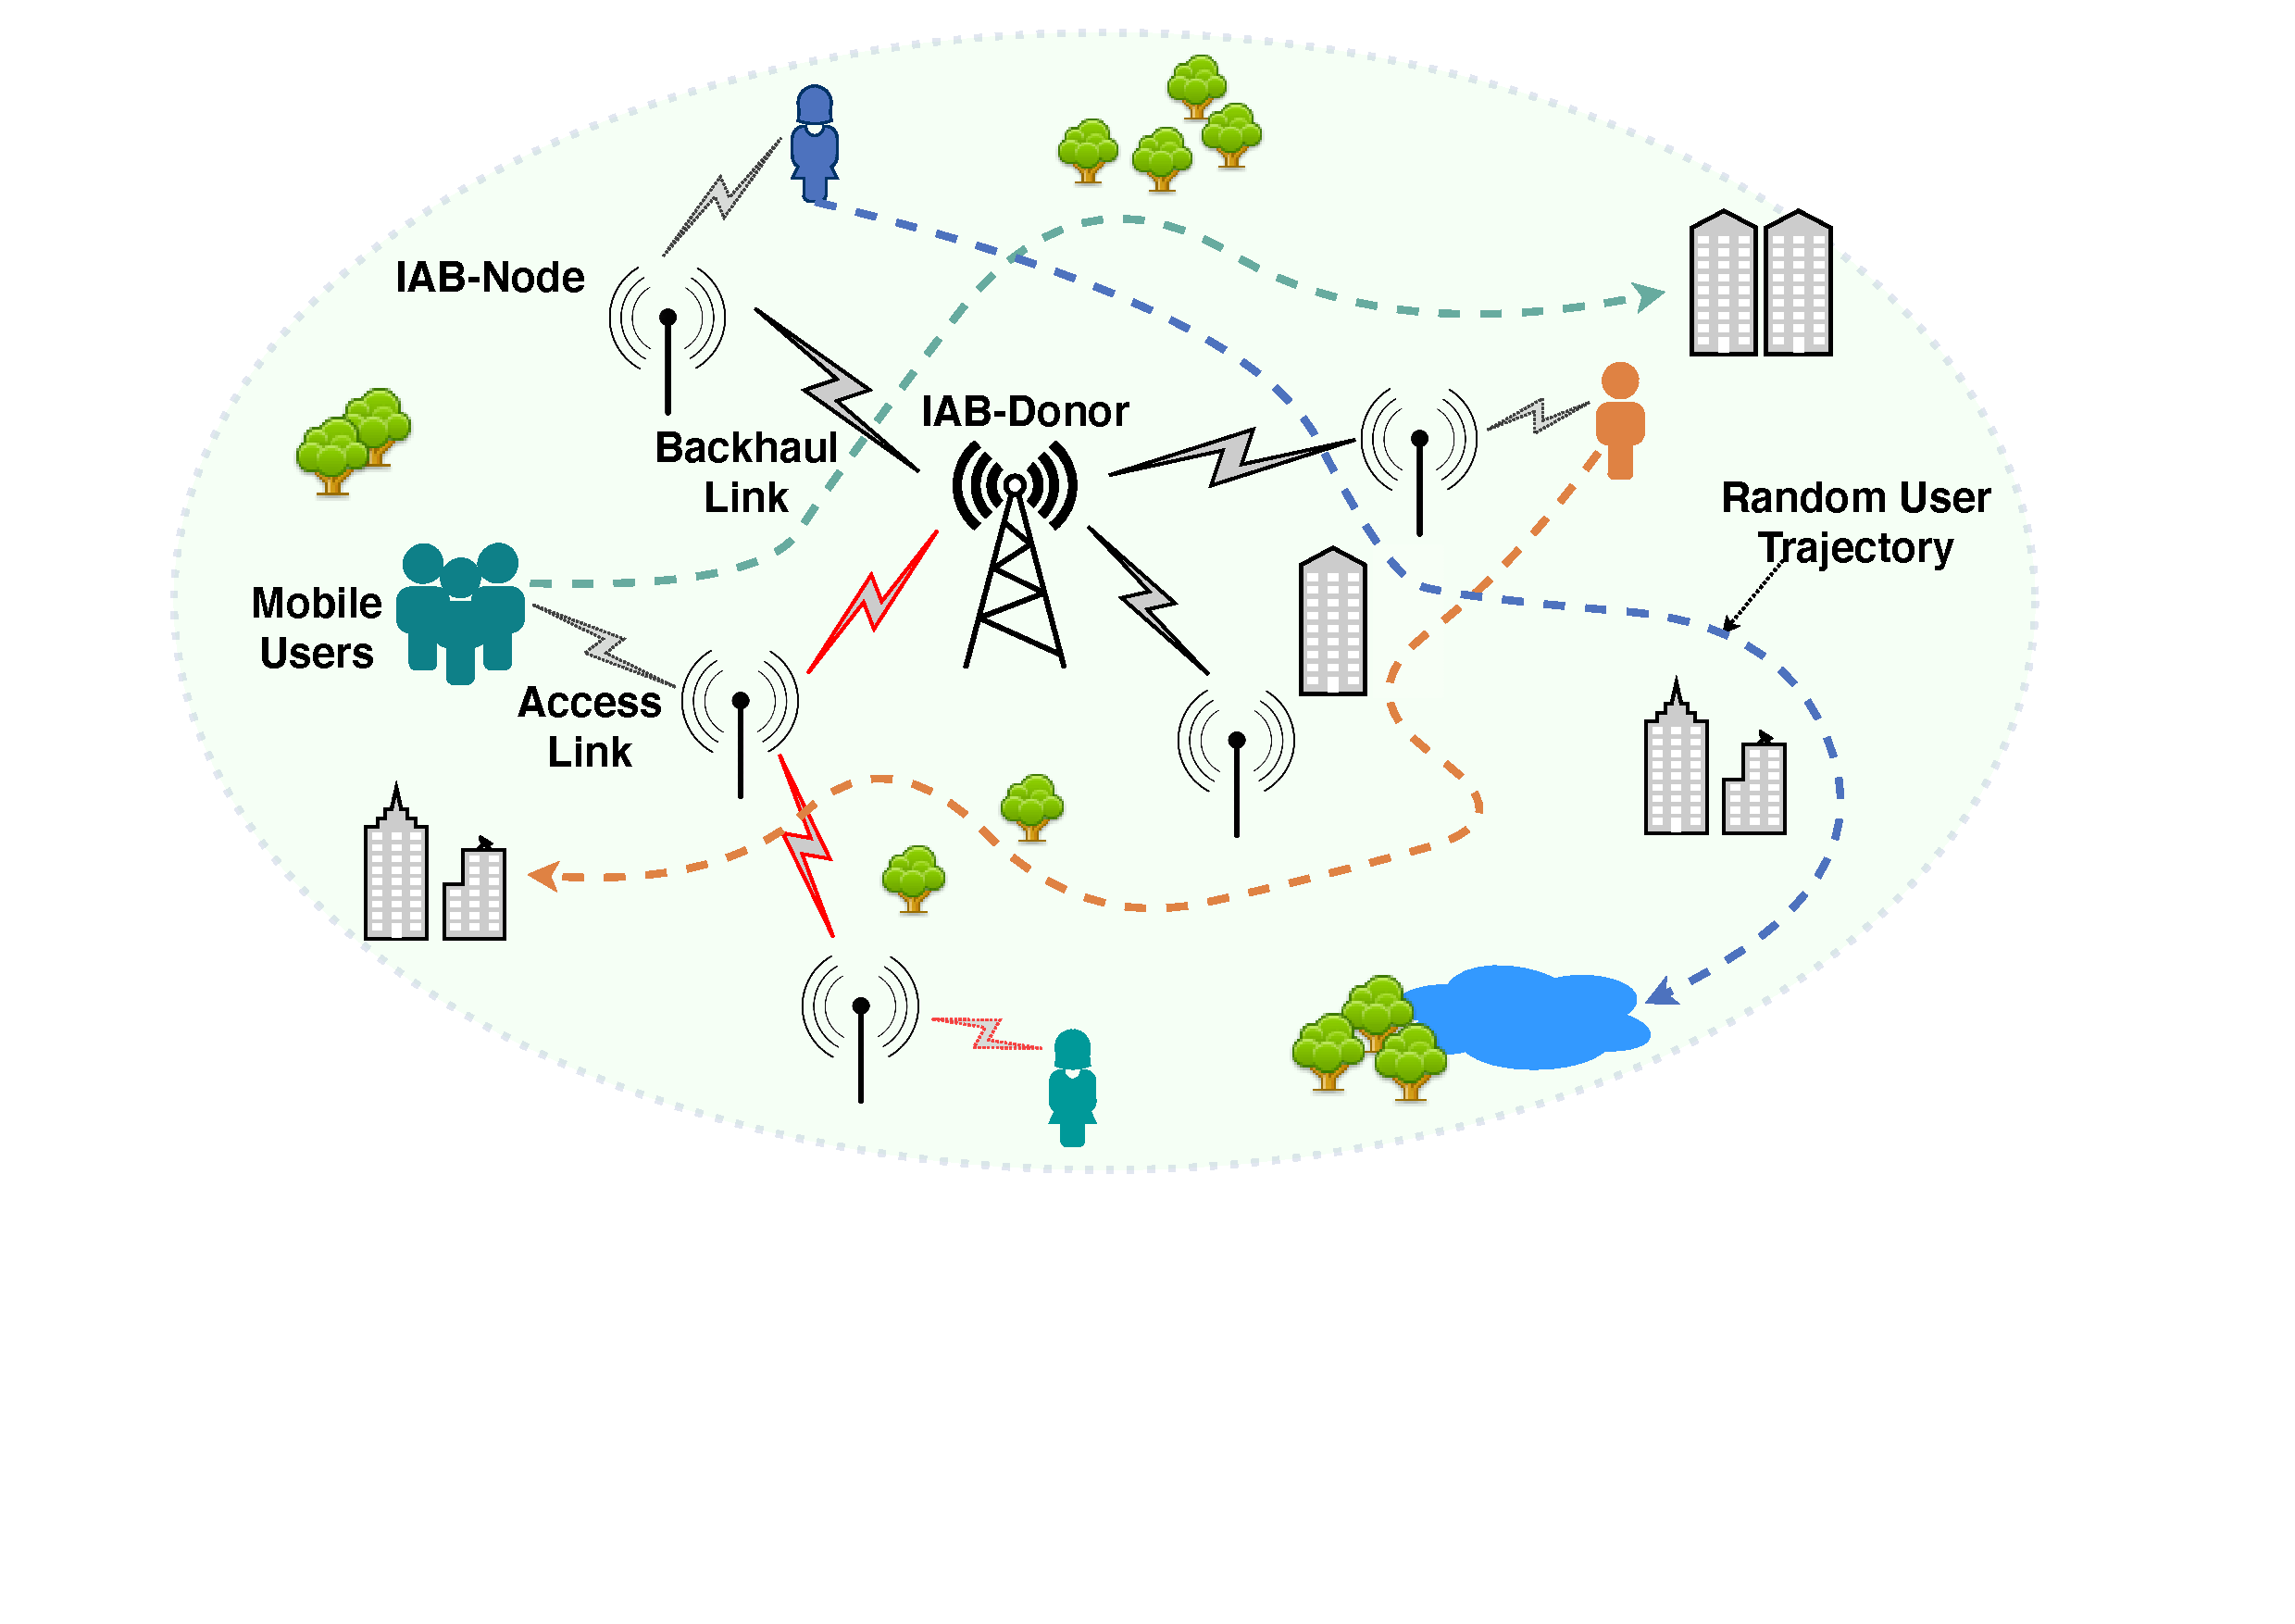
\includegraphics[width=0.4\textwidth]{figures/scenario.pdf}
	\caption{\small An example of IAB network scenario with mobile users. The dashed arrows represent user trajectories.}
	\label{fig:scenario}
	\vspace{-6mm}
\end{figure}

This scenario can be represented as a graph $\mathcal{G(\mathcal{V}, \mathcal{E})}$ where the node set $\mathcal{V}$ consists of an IAB-donor, IAB-nodes and UEs, and the edge set $\mathcal{E}$ includes all the potential links among the nodes. $\mathcal{V}$ can be further divided into the set of IAB-nodes $\mathcal{R}$ and the set of UEs $\mathcal{U}$. If not differently specified, the IAB-donor is identified as a special IAB-node.
We consider a tree topology for the backhaul network, where IAB-nodes are connected to the IAB-donor either directly or via multiple hops, as indicated in 3GPP specifications for IAB networks \cite{3gpp14studyPhysical}, which assume no more than 10 IAB-nodes organized in simple topologies.



\subsection{Channel Model}
\label{blockage_mobility_model}

We adopt typical path loss and antenna pattern models \cite{maltsev2014d5} for mmWave communications. The path loss model, considering both the line-of-sight (LOS) component and close reflections from the ground and other objects, is defined as \cite{maltsev2014d5} Eq. 5-37:
\begin{equation}
	PL_{dB} = \alpha + k\cdot10\cdot \text{Log}\left(\frac{d}{d_0}\right),
	\label{pathloss}
\end{equation}
where $\alpha=82.02dB$ and $d_0=5m$. $d$ is the path length. The propagation factor $k$ is 2.36 if $d > d_0$ and 2 otherwise.
The antenna gain is modeled with a Gaussian main lobe profile \cite{maltsev2014d5} Eq. 5-32:
\begin{equation}
	G_{dB}(\phi, \theta) = 10\cdot\text{Log}(G_0) - 12\cdot\frac{\phi^2}{\phi^2_{-3dB}} - 12\cdot\frac{\beta^2}{\beta^2_{-3dB}},
	\label{antenna_gain}
\end{equation}
\begin{equation}
	G_0 = \frac{16\pi}{6.76\cdot\phi_{-3dB}\cdot\beta_{-3dB}}.
 \label{base_antenna_gain}
\end{equation}
$\phi_{-3dB}$ and $\beta_{-3dB}$ are respectively the elevation and azimuth half power beam widths (HPBWs). The $\phi$ and $\beta$ are the elevation and azimuth angle offsets between the main lobe direction and the direction to the considered transmitter/receiver.
A visible definition of $\phi_{-3dB}$, $\beta_{-3dB}$, $\phi$ and $\beta$ can be found in Figs. 5-18, 5-19 and 5-20 in \cite{maltsev2014d5}.

Non-line-of-sight (NLOS) conditions are mainly caused by blocking obstacles. IAB-nodes are expected to be installed at relatively high places (e.g., street lights, roof tops, etc.) to improve visibility and avoid tampering (e.g., the height of IAB-nodes is typically assumed to be about $6$m, which is hard to be reached even for a double-decker bus), thus we expect that mobile obstacles can rarely affect backhaul links. Nevertheless, there can still be some static obstacles, such as buildings, causing severe blockages to backhaul links. However, they can be effectively avoided in the network planning stage by considering radio coverage.
In contrast, access links are exposed to more recurrent blockages caused by nomadic obstacles (e.g., pedestrian, transportation traffic, etc.). Based on these observations, we realistically apply random and mobile obstacle blockages only to access links.

We consider 3D mobile obstacles \cite{gapeyenko2017temporal} that move
according to Random Waypoint model \cite{bai2004survey}.
Fig. \ref{fig:3d_blockage}(a) shows an example  of how the blockage between a transmitter and a receiver occurs.
An obstacle is modeled as a cylinder standing in the LOS path between the transmitter and the receiver.
Fig. \ref{fig:3d_blockage}(b) shows the corresponding top view where the intersection points between the LOS path and the blocking cylinder are identified as $A$, $B$ and $C$, having respectively heights of $h_A$, $h_B$ and $h_C$. To determine whether a link blockage occurs, the following cases, represented in Fig. \ref{fig:3d_blockage}(b), are examined:
\begin{itemize}
	\item Case \Romannum{1}: when the LOS path is neither a secant nor a tangent of the blocker's cross-section, there is no blockage in the transmission.
	\item Case \Romannum{2}: when the LOS path is a tangent of the blocker's cross-section, if $h_A \leq h_{block}$, the blockage occurs; otherwise, no blockage occurs.
	\item Case \Romannum{3}: when the LOS path is a secant of the blocker's cross-section. A blockage occurs only if $h_B \leq h_{block}$ or $h_C \leq h_{block}$.
\end{itemize}
Every time an obstacle interrupts a transmission, the link blockage occurs according to a knife-edge diffraction model indicated in the 3GPP specification \cite{3gpp15studyChannel}, where the additional attenuation caused by each obstacle is applied to the path loss model \eqref{pathloss}.
We would like to remark that the above models are just reasonable choices to obtain realistic scenarios, and thus meaningful numerical results. Indeed, the approach we propose can be applied to other specific path loss, antenna pattern and blockage models as well.

\begin{figure}
	\centering
 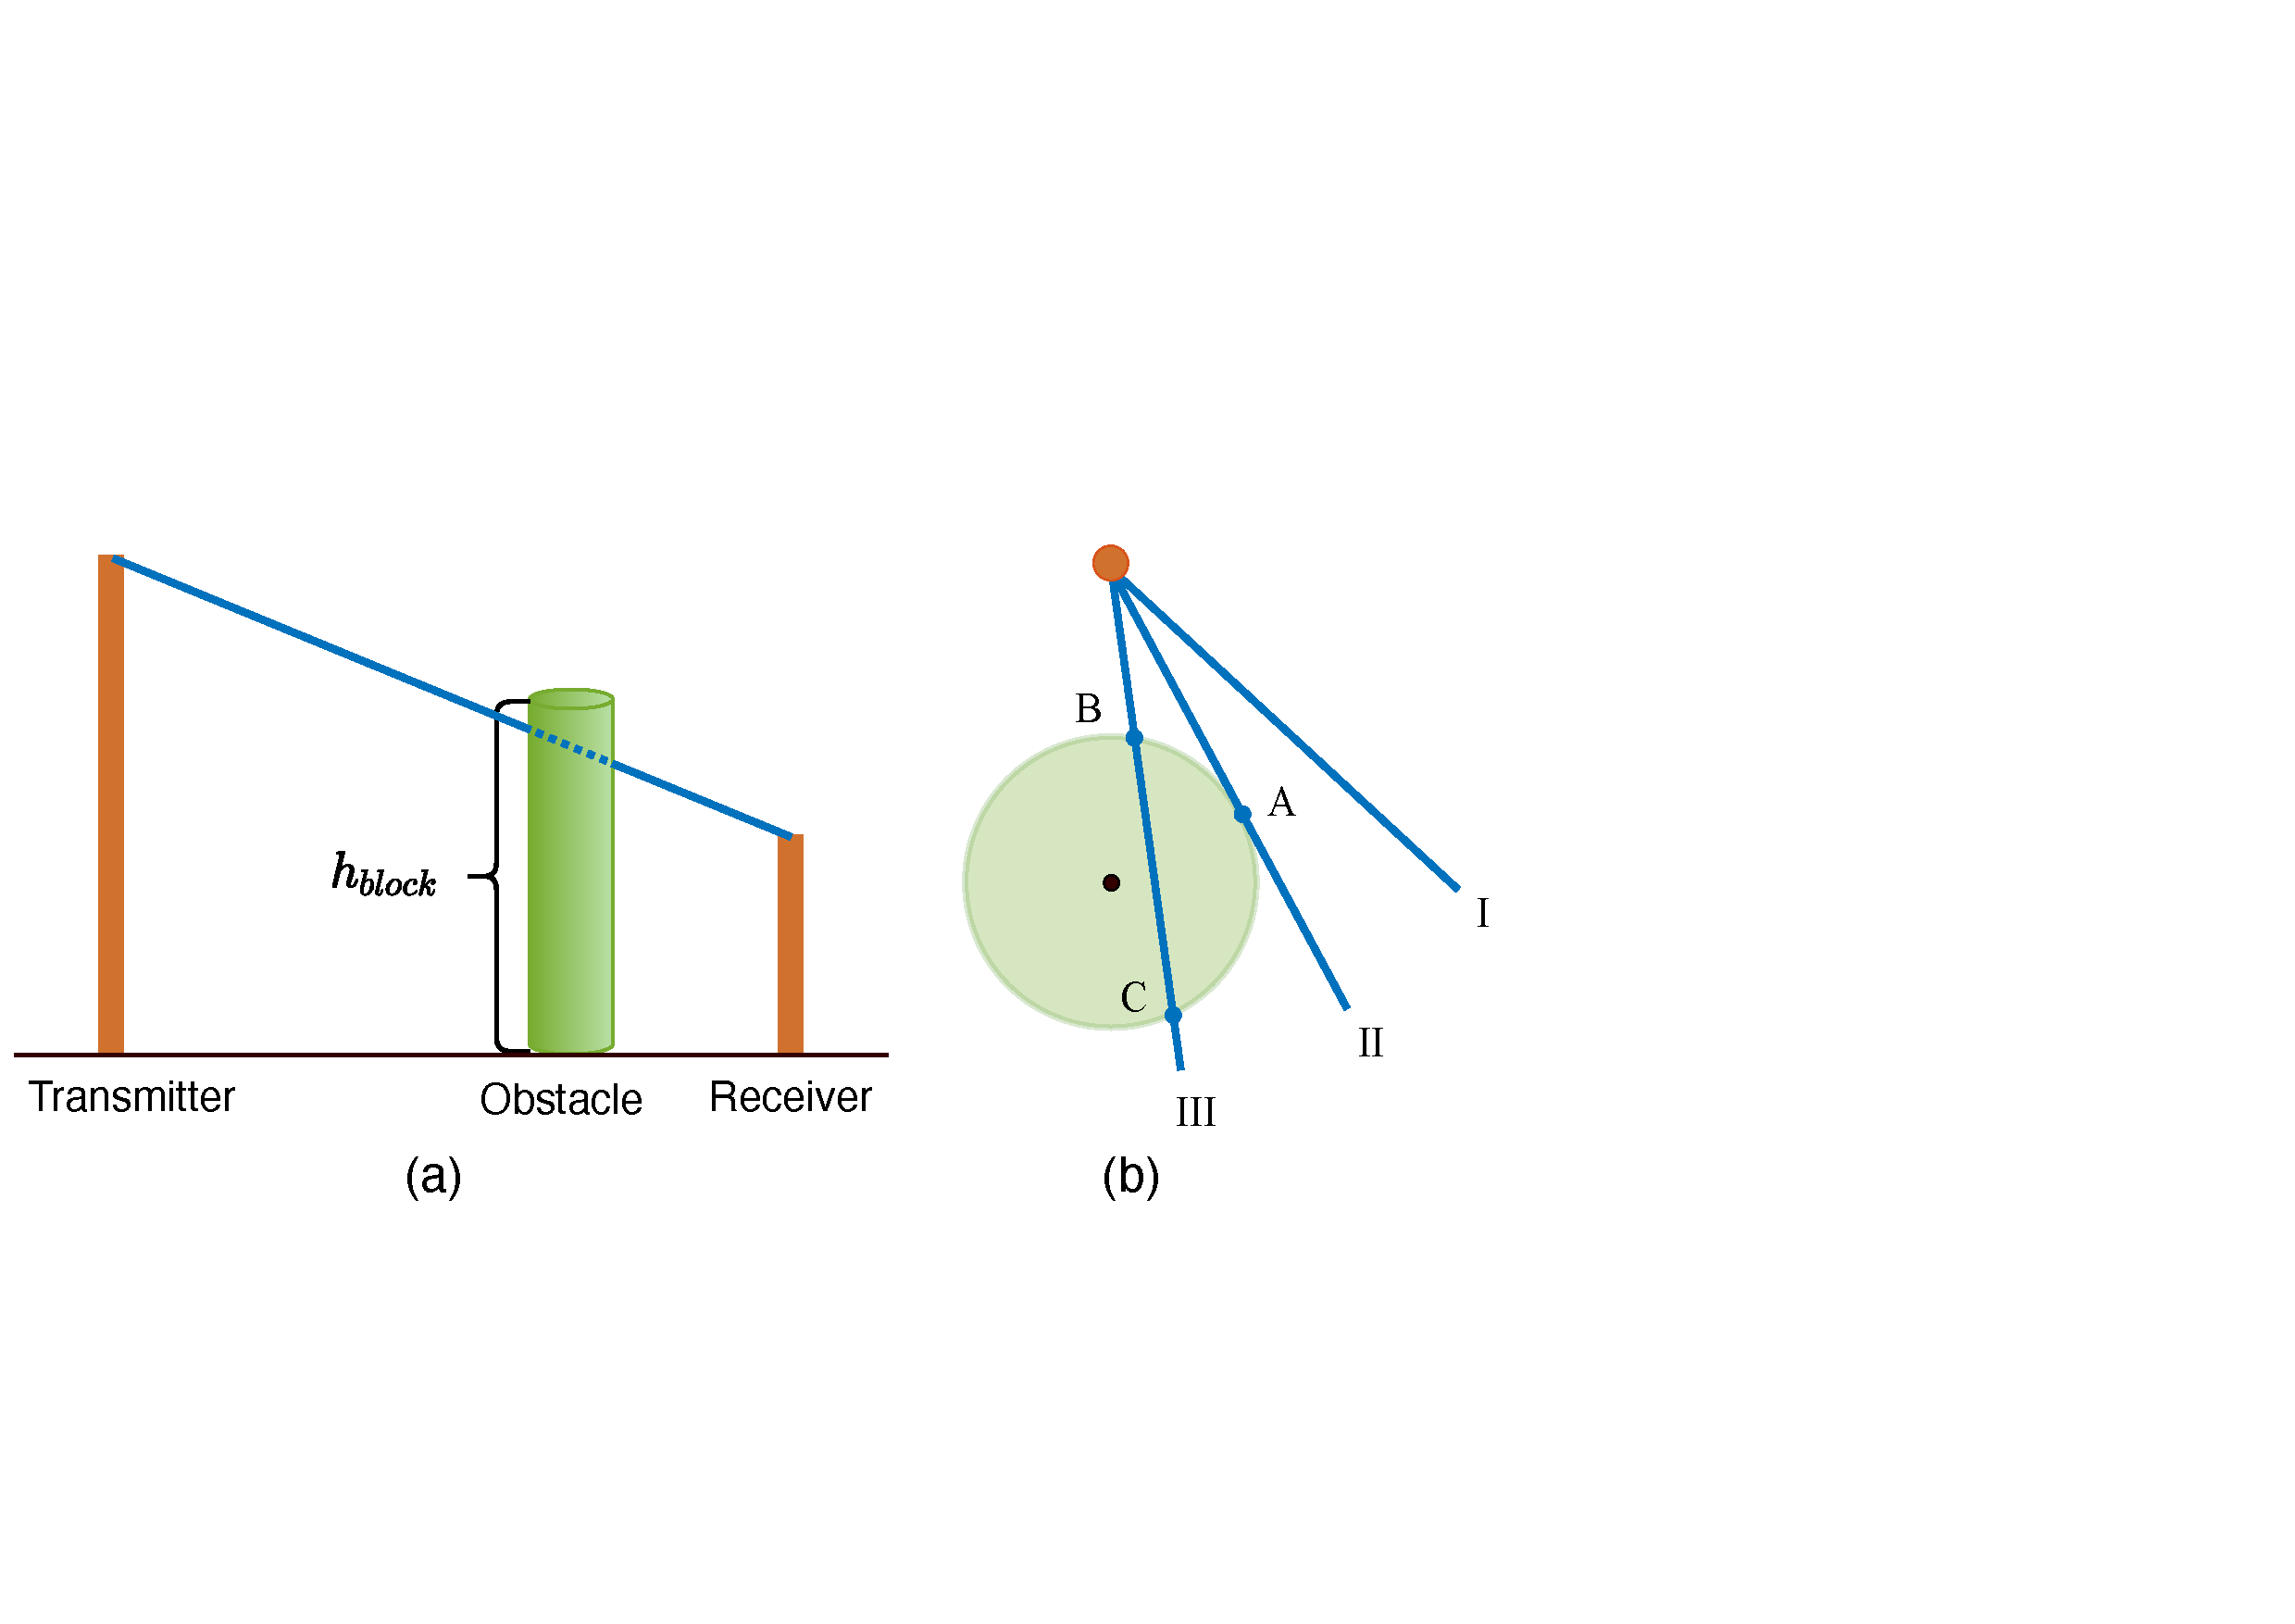
\includegraphics[width=0.45\textwidth]{figures/TON_revision/3d_blockage_model.pdf}
	\caption{\small Blockage model considering 3D obstacles.}
	\label{fig:3d_blockage}
	\vspace{-4mm}
\end{figure}

\subsection{Network Designs}

In this work, we aim to investigate downlink traffic transfer from the IAB-donor to UEs, in order to provide maximum UE throughput in IAB networks with the following designs. 
All the IAB-nodes together operate either in HD mode (i.e., either receiving or transmitting data in the same slot) or in FD mode (i.e., able to simultaneously receiving and transmitting data). An HD IAB-node (or IAB-donor) is equipped with $N_p$ side-by-side array panels that simultaneously manage transmission (Tx) and reception (Rx), while a FD IAB-node is equipped with $N_p$ side-by-side pairs of separate Tx and Rx array panels\footnote{In the experiments carried out in Sec.~\ref{experiments}, we assume ideal self-interference cancellation and isolation for FD IAB-nodes, however, the proposed approach can also be applied in scenarios where self-interference is included, but with a potential performance degradation.}\cite{xiao2017full}. We employ uniform planar arrays (UPAs) with codebook-based beamforming as panel antenna arrays, each of which covers a $180^\circ$ area that is divided into $N_s$ sectors indicating possible beam directions. Each array panel is equipped with a single radio frequency (RF) chain thus able to create and process one baseband data stream, scheduling different single-beam at different panels. Therefore, an IAB-donor or IAB-node can process a total of $N_p$ baseband streams at a time. Fig. \ref{fig:principle}(b) provides an example of the top view of a node.
Based on the above designs, the IAB networks are deployed in the following.

In the \textit{backhaul}, two endpoints of a backhaul link point each other using the reciprocal sector and panel whose normal direction is the closest to the one of the LOS segment, as shown with the dashed lines in Fig.~\ref{fig:principle}(a) that depicts an example of an IAB wireless backhaul.
Nodes in the backhaul are equipped with buffers of unlimited size. As this work focuses only on the IAB networks, to eliminate the effect of traffic dynamics in the core network, we assume the IAB-donor's buffer to always store sufficient data\footnote{In this work, data flows are not differentiated and prioritized over different users, but regarded as equivalent for all users that are interested in the same data.}
to be delivered.
Each IAB-node holds a buffer storing the bits received via backhaul links from its parent. The buffers could be the bottleneck of multi-hop transmissions. \begin{changed}Indeed, if a buffer is empty, the activated links will transmit nothing and thus it causes a downlink starvation problem.\end{changed}
Therefore, the flow routing and link scheduling scheme is expected to timely refill the buffers to avoid any impact of the little amount of cached bits on downstream transmissions.

In the \textit{access}, UEs connecting to such a backhaul are associated to sectors based on their positions. A UE can belong to two sectors if it is located on a sector boundary. And UEs are expected to work in a dual-connectivity mode \cite{polese2017improved}, i.e., equipped with both legacy (3GPP FR1) and mmWave (3GPP FR2) interfaces. It is arguable that control-plane information can be exchanged through legacy FR1 interfaces to provide better coverage and signal propagation conditions.
Then, the control-plane FR1 interface can be used to send UE context information to enable better network access selection and configuration.
Therefore, we assume that each IAB-node is informed about associated UEs in real time and their channel status. Channel status information is typically available at each BS via Reference Signals and used for beamforming, rate adaptation, and other 5G procedures. BSs can also estimate the number and the position of connected UEs by activating network-side ranging techniques \cite{bernazzoli20235g}.
Instead, high-throughput user-plane channels can be established through mmWave (FR2) links.

The time domain $\mathcal{T}$ is divided into frames, each of which consists of $T$ slots of equal length $\delta$. 
The system, following a space-division multiple access (SDMA) scheme based on beamforming, takes advantage of the high directivity of mmWave antennas and can allow multiple concurrent transmissions, both backhaul and access links, to be carried out in each slot, by sharing the radio resources and carrying out transmissions through beams at different panels.
The simultaneous activation of several links requires the network to satisfy physical requirements, such as channel conditions (e.g., interference levels, antenna patterns), duplexing modes (i.e., FD, HD), RF chain limitations, UE hardware limitations, etc.
Signal-to-interference-plus-noise ratio (SINR) model is adopted to establish a successful link: a connection is created only if the SINR at the receiver is larger than the threshold required by the selected modulation and coding scheme (MCS). The interference that one link receives is the sum of the power it receives from all the non-intended transmitters simultaneously activated. Rate adaptation is considered as well, i.e., transmission rates depend on selected MCSs, which in turn depend on achievable SINR values.

\subsection{Network Operations}
\label{network_operations}

The transmissions follow and satisfy the rules and constraints below. A parent IAB-node -- more specifically, its RL agent(s) -- will have to choose between (1) sending data bits to a child IAB-node via a \textit{backhaul} link to refill its buffer, and (2) directly transmitting to a UE via an \textit{access} link to myopically improve its throughput. For a \textit{backhaul} transmission, if an IAB-node working in HD mode is selected as a receiver of its parent node in a specific slot, it cannot transmit in the same slot. For an \textit{access} transmission, a UE can be selected as a receiver if a beam points to its located sector. If more than one UE is present in the sector, one of them is randomly selected as the intended receiver.
Due to hardware limitations, a UE can receive from at most one IAB-node / IAB-donor in a slot, therefore, a collision occurs if a UE is selected as a receiver from more than one panel (i.e., more than one IAB-node) in the same time slot. Whenever it occurs, no bit can be delivered to the UE.
For both \textit{backhaul} and \textit{access} transmissions, if the amount of data bits cached in a buffer, rather than the link capacity, is the limiting factor, the outgoing links simultaneously activated equally share buffered bits to pursue the fairness.




The mmWave access network scenario above described is characterized by UEs moving with arbitrary directions and speeds, which may undergo link blockages caused by random mobile obstacles. This makes access links short-lived and unstable. In order to address such dynamics, in the next sections, we propose an adaptive MARL-based flow routing and link scheduling approach.


\begin{figure*}[ht]
	\centering
	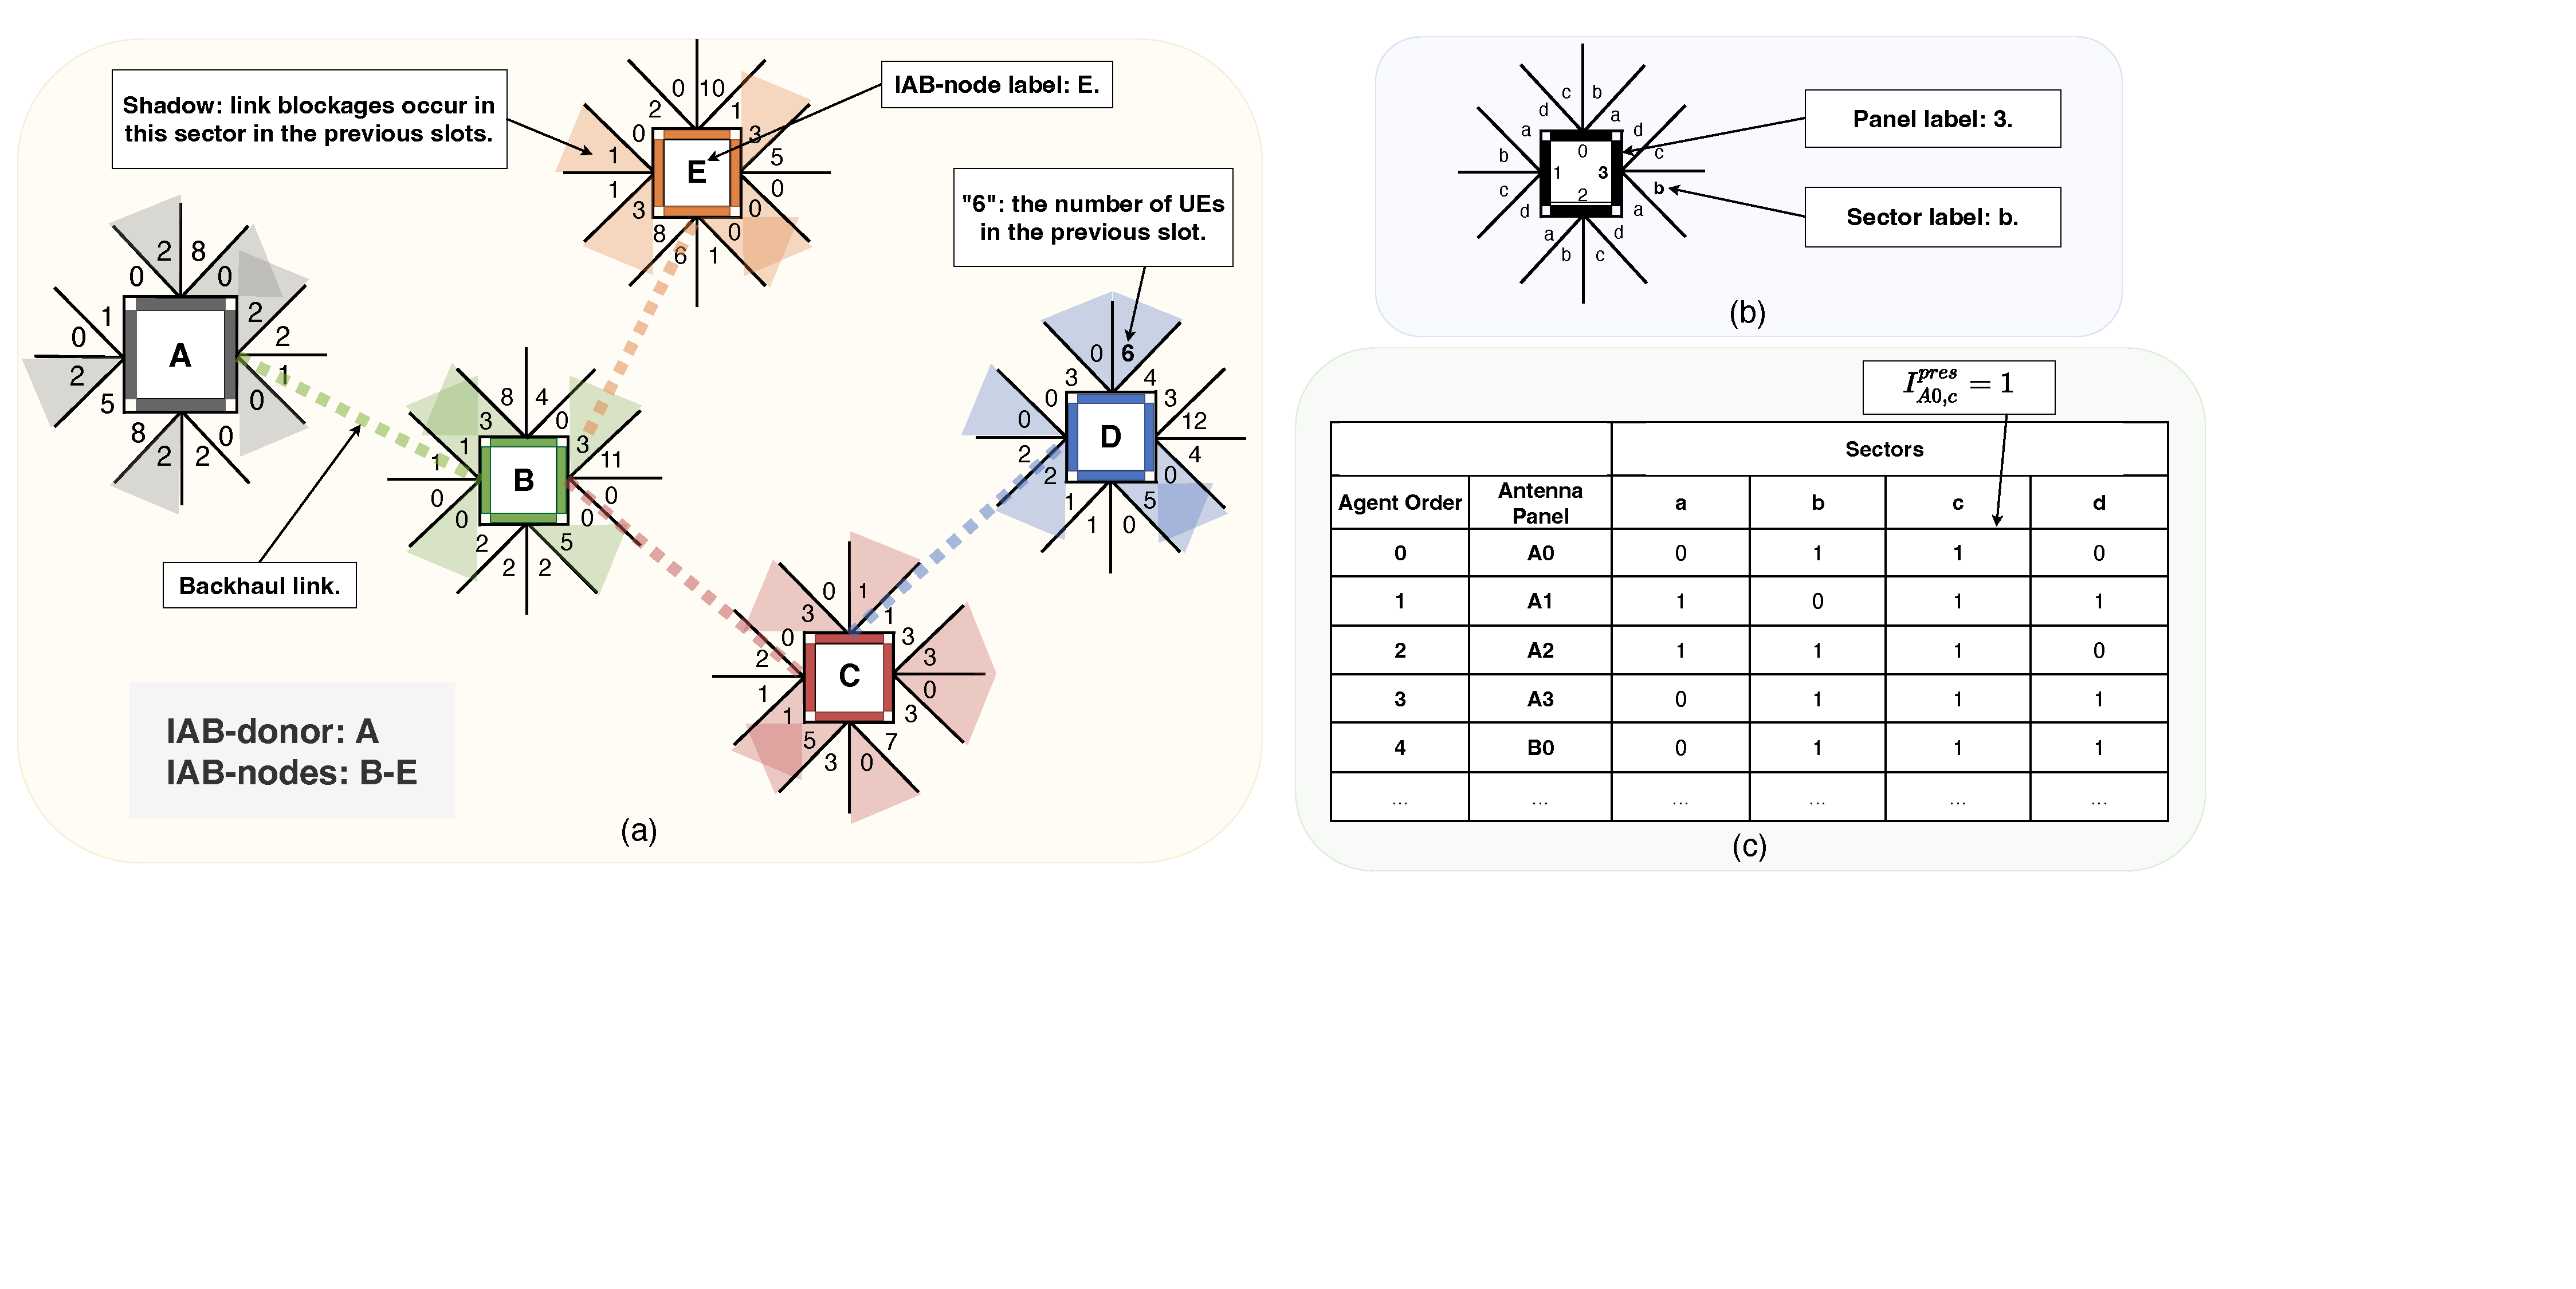
\includegraphics[width=0.8\linewidth]{figures/revision/principle.pdf}
	\caption{\footnotesize A top-view example of IAB network scenario and its corresponding RL formulation. \textbf{(a)} shows an IAB network with 1 IAB-donor and 4 IAB-nodes. Backhaul links (dashed lines) form a tree topology and the number of covered UEs is reported in each sector. A sector is shadowed if blockages have been detected in it in the previous slots. \textbf{(b)} details an IAB-node equipped with $N_p=4$ Tx array panels (1, 2, 3, 4), each of which manages $N_s=4$ sectors (a, b, c, d). \textbf{(c)} includes a table recording the binary UE presence information for the sectors shown in (a).
	}
	\label{fig:principle}
    \vspace{-4mm}
\end{figure*}

\setlength{\textfloatsep}{6pt}
\begin{table}[!h]
\scriptsize
    \caption{\small Summary of notations in Sections \ref{system_model} and \ref{method}.}
    \label{notation_1}
    \centering
    \begin{tabular}{@{\hspace{1pt}} l @{\hspace{1pt}} l}
        \toprule
        Notations & Definitions \\
        \midrule
        $\mathcal{G},\mathcal{V},\mathcal{E}$ & Network graph, node set, and edge set\\
        $\mathcal{R},\mathcal{U}$ & The set of IAB-nodes (including IAB-donor), and set of UEs\\
        $\mathcal{T},T,\delta$ & Time domain, the number of slots in a frame, and slot length\\
        $PL_{dB},G_{dB}$ & Path loss, and antenna gain\\
        $\phi_{-3dB}$ & Elevation HPBW\\
        $\beta_{-3dB}$ & Azimuth HPBW\\
        $N$ & The total number of RL agents (antenna array panels)\\
        $N_p,N_s$ & The No. of panels per IAB-node, and No. of sectors per panel\\
        $\mathcal{I}_p,\mathcal{I}_s$ & The sets of indicies for panels and sectors per panel\\
        $\mathcal{O},\mathcal{A},\pi$ & Observation space, action space and policy\\
        $o_t,a_t,r_t$ & Observation, action and reward at step $t$\\
        $o^{(i)}_t,r^{(i)}_t$ & The agent (panel) $i$'s observation and reward at step $t$\\
        $I^{pres}_{i,s}$ & Indicator of whether there are UEs in sector $s$ of agent (panel) $i$\\
        $A^{block}_{i,s}$ & Indicator of accumulated attenuation in sector $s$ of agent (panel) $i$\\
        $\mathcal{R}_i$ & The set of child IAB-nodes of agent (panel) $i$\\
        $L_n$ & The number of bits cached on the IAB-node $n$\\
        $B^N_n$ & The number of bits transmitted by the IAB-node $n$\\
        $B^P_i$ & The number of bits transmitted by the agent (panel) $i$\\
        $h(i)$ & The number of hops to reach agent (panel) $i$ from the IAB-donor\\
        $c_{min}$ & The minimum capacity available in the whole network\\
        $\rho_{BH}$ & The weight to counterbalance the large backhaul link capacity\\
        $\mathcal{I}_p^{EB}$ & The set of
panels with empty buffers\\
        $\mathcal{I}_p^{RX}$ & The set of panels whose located IAB-nodes are receiving data\\
        $\mathcal{I}_p^{ER}$ & The union of $\mathcal{I}_p^{EB}$ and $\mathcal{I}_p^{RX}$\\
        $\zeta$ & The penalty term in the reward function \\
        \bottomrule
    \end{tabular}
\end{table}